%%%%%%%%%%%%%%%%%%%%%%%%%%%%%%%%%%%%%%%%%%%%%%%%%%%%%%%%%%%%%%%%%%%%%%
% How to use writeLaTeX:
%
% You edit the source code here on the left, and the preview on the
% right shows you the result within a few seconds.
%
% Bookmark this page and share the URL with your co-authors. They can
% edit at the same time!
%
% You can upload figures, bibliographies, custom classes and
% styles using the files menu.
%
% If you're new to LaTeX, the wikibook is a great place to start:
% http://en.wikibooks.org/wiki/LaTeX
%
%%%%%%%%%%%%%%%%%%%%%%%%%%%%%%%%%%%%%%%%%%%%%%%%%%%%%%%%%%%%%%%%%%%%%%
\documentclass{tufte-handout}

%\geometry{showframe}% for debugging purposes -- displays the margins

\usepackage{amsmath}

% Set up the images/graphics package
\usepackage{graphicx}
\setkeys{Gin}{width=\linewidth,totalheight=\textheight,keepaspectratio}
\graphicspath{{graphics/}}

\title{Stata Lab 6: Visualization}
\author{DIME Analytics \\ dimeanalytics@worldbank.org}
% \date{24 January 2009}  % if the \date{} command is left out, the current date will be used

% The following package makes prettier tables.  We're all about the bling!
\usepackage{booktabs}

% The units package provides nice, non-stacked fractions and better spacing
% for units.
\usepackage{units}

% The fancyvrb package lets us customize the formatting of verbatim
% environments.  We use a slightly smaller font.
\usepackage{upquote}
\usepackage{fancyvrb}
\fvset{fontsize=\normalsize}
\renewcommand{\FancyVerbFormatLine}{\color{violet}}
\DefineShortVerb{\|}

% Small sections of multiple columns
\usepackage{multicol}

% Provides paragraphs of dummy text
\usepackage{lipsum}

% These commands are used to pretty-print LaTeX commands
\newcommand{\doccmd}[1]{\texttt{\textbackslash#1}}% command name -- adds backslash automatically
\newcommand{\docopt}[1]{\ensuremath{\langle}\textrm{\textit{#1}}\ensuremath{\rangle}}% optional command argument
\newcommand{\docarg}[1]{\textrm{\textit{#1}}}% (required) command argument
\newenvironment{docspec}{\begin{quote}\noindent}{\end{quote}}% command specification environment
\newcommand{\docenv}[1]{\textsf{#1}}% environment name
\newcommand{\docpkg}[1]{\texttt{#1}}% package name
\newcommand{\doccls}[1]{\texttt{#1}}% document class name
\newcommand{\docclsopt}[1]{\texttt{#1}}% document class option name

\begin{document}

\maketitle% this prints the handout title, author, and date

\begin{marginfigure}%
  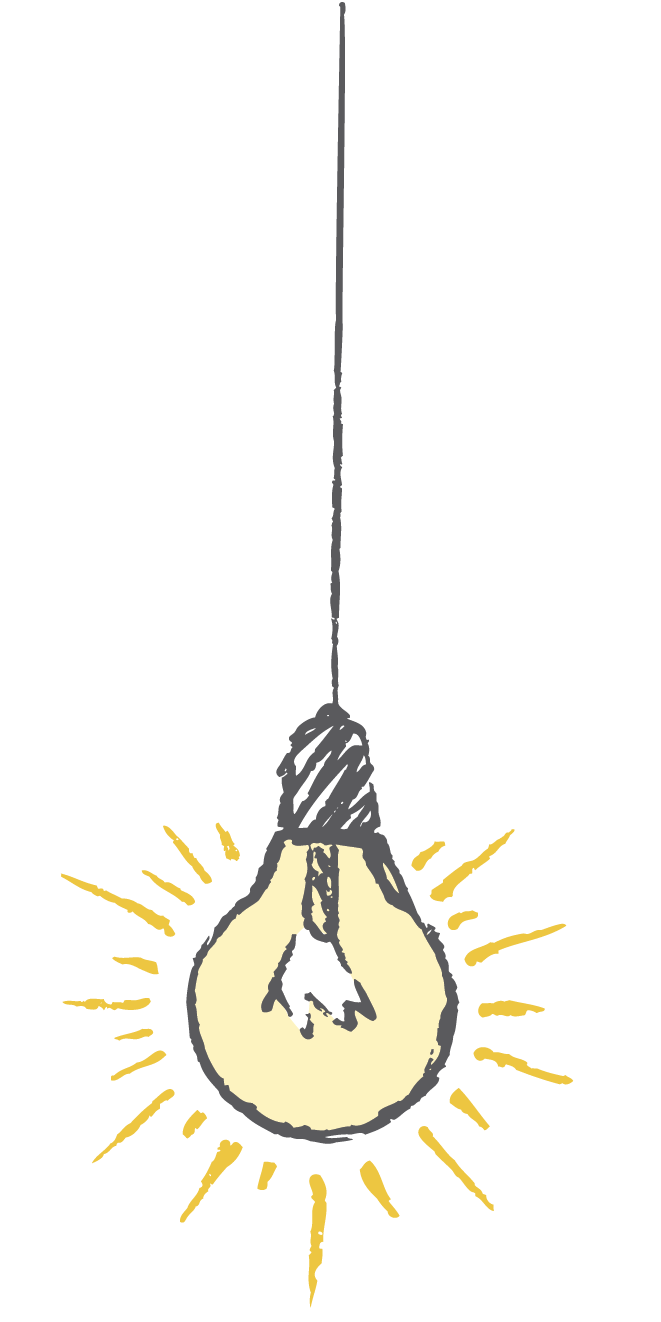
\includegraphics[width=\linewidth]{light.png}
\end{marginfigure}

\begin{abstract}
In this lab, we will learn to produce data visualizations in Stata.
These are figures that paint a picture of what a given dataset looks like.
These results begin to help us understand the important features of our dataset,
and can be useful in directing us towards areas for further analysis.

\bigskip\noindent \textbf{Exercise Objectives}:
\begin{enumerate}
  \item Learn how to produce and combine basic graph types
  \item Learn how to produce nice looking graphs
  \item Learn how to export graphs in common image formats
\end{enumerate}

\bigskip\noindent \textbf{Getting Started}:
\begin{enumerate}
 \item Open your |/DataWork/| folder for the full training. It should have subfolders for each of the Labs; if it does not, use |iefolder| to create the folder |/Lab6/| now.
 \item You will find a data file that we created in Lab 2, |hh_roster.dta| in the public Field Coordinator Training folder. Save this dataset to |/DataWork/Lab6/|.
 \item Visit \url{https://graykimbrough.github.io/uncluttered-stata-graphs/} and
 install the Uncluttered Graphs theme. This takes care of a lot
 of important graph defaults for you.
\end{enumerate}
\end{abstract}

%\printclassoptions
\section{Make a histogram}

A density plot like a histogram is often the first step to figuring out
what the distribution of critical variables looks like.
This exercise will introduce you to using a |histogram| command
on one variable and the styling commands needed to make a graph look good.

Create a new dofile and save it as |graphs.do|.
Start by loading only the data that represents households using the |tag_hh| variable.
Look at the variable |hh_ag_16_x_16_1|.
This is total days members of the household spent on land preparation.
First, use |histogram| to find a reasonable range over which to make a graph.
Once you have a good range, fix that range using |if|
(or change your subsetting in the |use| command).
Next, make the graph look nice.
Simple cleaning can go a long way.
Label the axes, color the bars, and see if there are any other
formatting options you'd like to change.
The Stata Graphics Manual is a great guide full of examples.
Finally, save the graph in |.gph| format.

\section{Make a bar chart}

Load the dataset. Now look at |hh_ag_16_x_16_2|,
a variable indicating whether or not the household hired labor to assist them.
Make sure this is a sensible variable in terms of categories
and extended value labels, then let’s find
out how this varied across cooperatives (|hh_gr_16|).
Use the |graph bar| command to plot the variation in the use of hired labor
across the different cooperatives.
Make the graph look nice using options and the |bar()| option,
then save it as a |.gph| file.

\section{Make a scatter plot with linear fits}

Load the dataset. Let’s see if there is a relationship between
the amount of time spent on land preparation and
hiring labor to help out, and if this varies by |treatment|.
These variables are |hh_ag_18_x_16_1| and |hh_ag_16_x_16_1|.
See how they correlate in the treatment and control groups.
Make a |tw| graph with four components:
\begin{enumerate}
  \item A scatter plot of the treatment group;
  \item a scatter plot of the control group; and
  \item and an |lfit| plot for each group overlaid.
\end{enumerate}
See if you can get the colors to correspond appropriately.
Save the graph as a |.gph| file.

\section{Combine and export all the graphs}

Use the |graph combine| command to put all three graphs on the same output.
See what different ways you can arrange them.
Since the combined graph is a final output, we will not save it as a |.gph| file.
Instead, we will use a production format like |.png| or |.eps|.
The |.png| format is usable for previews but is not suitable
for high-quality printing or journal production.
The |.eps| format can be expanded to any size,
and is also very lightweight for storage and backup,
but can't be previewed everywhere.
(It should work in modern version of Office, however.)

Thanks to the template creators.\cite{tuftelatex}

\bibliography{sample-handout}
\bibliographystyle{plainnat}

\newpage

\begin{figure*}[h]
\includegraphics{../DataWork/Lab6/histogram.eps}
\end{figure*}

\begin{figure*}[h]
\includegraphics{../DataWork/Lab6/lab6.eps}
\end{figure*}

\begin{figure*}[h]
{\setstretch{0.7}
\VerbatimInput[frame=lines,numbers=left,label=graphs.do]
{../DataWork/Lab6/graphs.do}}
\end{figure*}

\end{document}
